
%(BEGIN_QUESTION)
% Copyright 2012, Tony R. Kuphaldt, released under the Creative Commons Attribution License (v 1.0)
% This means you may do almost anything with this work of mine, so long as you give me proper credit

Et varmesystem for selvforsynte hjem er en {\it ekstern varmer}, der ved eller annet brensel brennes ved høy temperatur i korte perioder i en utendørs ovn. Varmen lagres i et stort ``termisk reservoar'' av sand. Ild tennes bare hver få dager, og varmen overføres til huset via vann i varmevekslere:

$$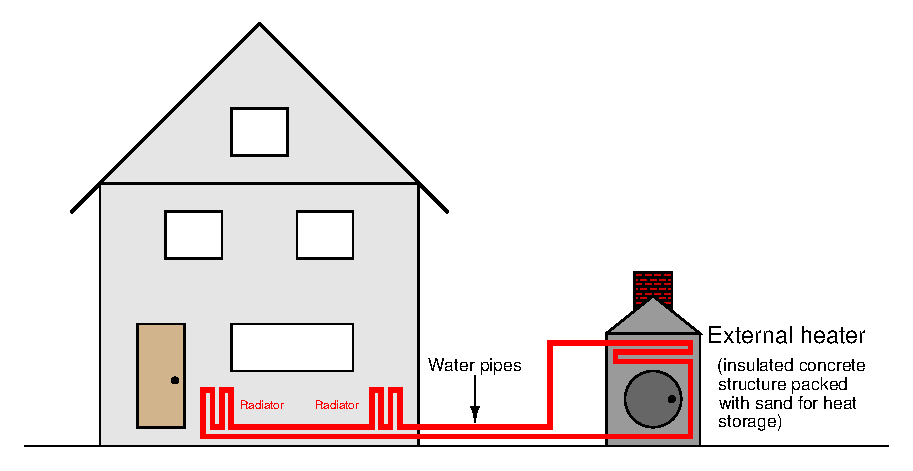
\includegraphics[width=15.5cm]{i01017x01.eps}$$

Svar på følgende spørsmål:

\begin{itemize}
\item{} Hvilke fordeler kan dette ha sammenlignet med ovn inne i huset?
\vskip 5pt
\item{} Hvorfor er {\it sand} et godt varmelagringsmedium?
\vskip 5pt
\item{} Er varmelagringen basert på {\it spesifikk varme} eller {\it latent varme}?
\vskip 5pt
\item{} Er varmeoverføringen i systemet basert på {\it spesifikk varme} eller {\it latent varme}?
\vskip 5pt
\item{} Hvordan kan hustemperaturen reguleres termostatisk?
\vskip 5pt
\item{} Hvordan kan systemet utstyres med alarm for ny opptenning?
\vskip 5pt
\item{} Beregn entalpien til vannet inn til huset ved 184 $^{o}$F.
\vskip 5pt
\item{} Beregn entalpien til vannet ut fra huset ved 127 $^{o}$F.
\vskip 5pt
\item{} Beregn varmeeffekten til huset ved vannmasseflow 9.2 lb/min.
\end{itemize}

\underbar{file i01017}
%(END_QUESTION)





%(BEGIN_ANSWER)

\begin{itemize}
\item{} Fordeler: {\it sikkerhet, høy forbrenningseffektivitet, og praktisk drift med sjeldnere fyring}.
\vskip 5pt
\item{} Sand er godt egnet fordi den {\it ikke smelter/fryser/lekker, har høy tetthet og brukbar varmekapasitet}.
\vskip 5pt
\item{} Varmelagringen er basert på {\it spesifikk varme}.
\vskip 5pt
\item{} Varmeoverføringen til huset er også {\it spesifikk varme} (vannet koker ikke).
\vskip 5pt
\item{} Termostat kan sykle pumpen som sirkulerer vann mellom ovn og hus.
\vskip 5pt
\item{} Lavtemperaturalarm med sensor i sandreservoaret kan varsle behov for ny opptenning.
\vskip 5pt
\item{} Entalpi inn ved 184 $^{o}$F: {\it 152 BTU/lb}.
\vskip 5pt
\item{} Entalpi ut ved 127 $^{o}$F: {\it 95 BTU/lb}.
\vskip 5pt
\item{} Varmeeffekt: {\it $(152-95)\times 9.2 = 524.4$ BTU/min = 31,464 BTU/h}.
\end{itemize}


%(END_ANSWER)





%(BEGIN_NOTES)

$$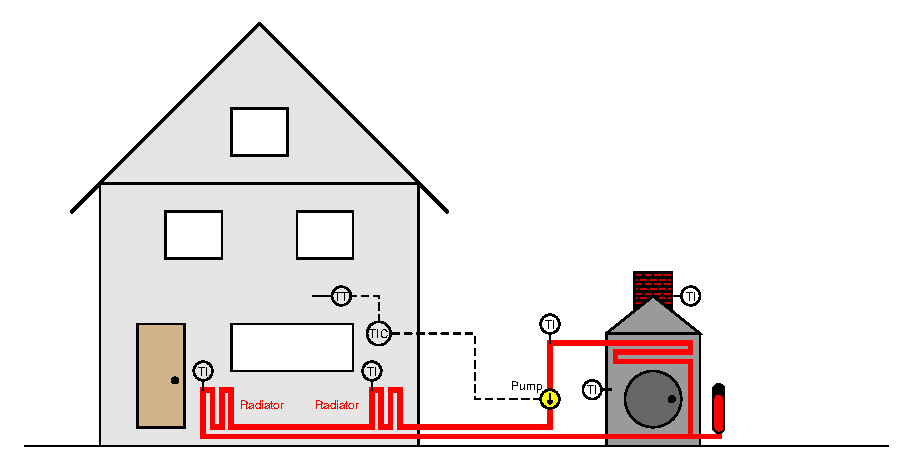
\includegraphics[width=15.5cm]{i01017x02.eps}$$

\vskip 20pt \vbox{\hrule \hbox{\strut \vrule{} {\bf Virtuell feilsøking} \vrule} \hrule}

Denne oppgaven egner seg godt for virtuell feilsøking med symptomer og foreslåtte tester.

\begin{itemize}
\item{} Hva forteller resultatet av siste test om feilen?
\item{} Hvis siste test ga et annet resultat, hva ville det betydd?
\item{} Er siste test den beste mulige testen?
\item{} Hva er ideell testrekkefølge for færrest steg?
\end{itemize}

%INDEX% Measurement, heat: conduction through a solid substance
%INDEX% Physics, heat and temperature: desuperheating

%(END_NOTES)

